\documentclass[10pt]{article}

\usepackage{amsmath}
\usepackage{amssymb}
\usepackage{graphicx}

\pagestyle{plain}

\setlength{\textwidth}{6.5truein}
\setlength{\textheight}{8.7truein}
\setlength{\oddsidemargin}{2.0mm}
\setlength{\evensidemargin}{2.0mm}
\setlength{\marginparwidth}{20pt}
\setlength{\topmargin}{-24.5truemm}
\setlength{\parindent}{0.0truemm}
\parskip=0.5mm

\title{\bf DECO3801 Executive Summary}
\author{\normalsize THEM - Typed HTML5 Evaluation Machine \\ \normalsize Carl Hattenfels, Scott Heiner, Shen Yong Lau, Robert Meyer, Brendan Miller, David Uebergang}
\date{}

\begin{document}

\maketitle

\section*{The Product - Typed HTML5 Evaluation Machine}

\subsection*{What is it?}

The Typed HTML5 Evaluation Machine is a web application, designed to allow users to upload and verify their HTML5 code. It also aims to provide helpful feedback so the users can learn what they did wrong, and improve on their mistakes. This project had been provided by client Lorna MacDonald, who runs the introductory web design course at the University of Queensland, understanding that the web standard was moving to HTML5. She had seen no validators online that filled the function of not just informing users about their HTML errors, but helped them to fix and improve on these errors, not to mention very few validators that actually validated according to the HTML5 specifications. It uses php, Javascript and XHTML for the website, and was developed with an interchangeable Python parsing back-end that communicates with the website through JSON-RPC.

\subsection*{How can it be used?}

Users are able to directly type their HTML code into the system, upload full files, and validate whole websites. The user is then shown their HTML code complete with information about general errors about what the code is missing, and sections of the code highlighted that are incorrect. Four different colours are used to refer to four different types of errors:

\begin{center}

\includegraphics[scale=0.5]{errortypes.png}
\end{center}

Structural and semantic errors are those that affect how your webpage is seen, while Accessibility errors are relevant to cover all web users, including the blind. Deprecated errors refer to tags that no longer perform as expected by all browsers, and will likely be phased out in the next web standard. The remaining errors are cases of Poor Practice which are less pertinent than the other errors but still important to achieve best practices.

\begin{center}
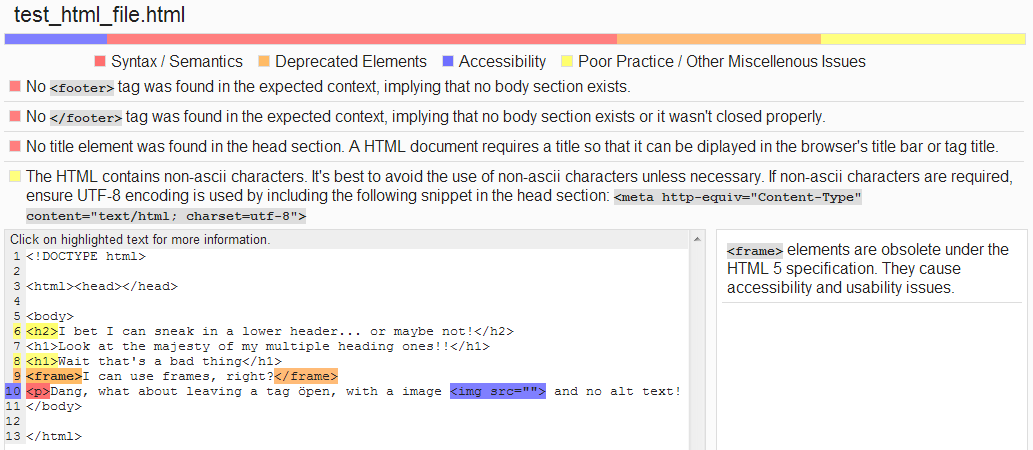
\includegraphics[scale=0.3]{output_highlighting.png}
\end{center}

You can see the highlighted sections above. Users are able to click on these highlighted sections to find out more about the error, and understand where they've gone wrong. For example, the selected \verb+<frame>+ tag is deprecated and should be avoided. The selected tag is bolded to highlight which one the user has selected.

\begin{center}
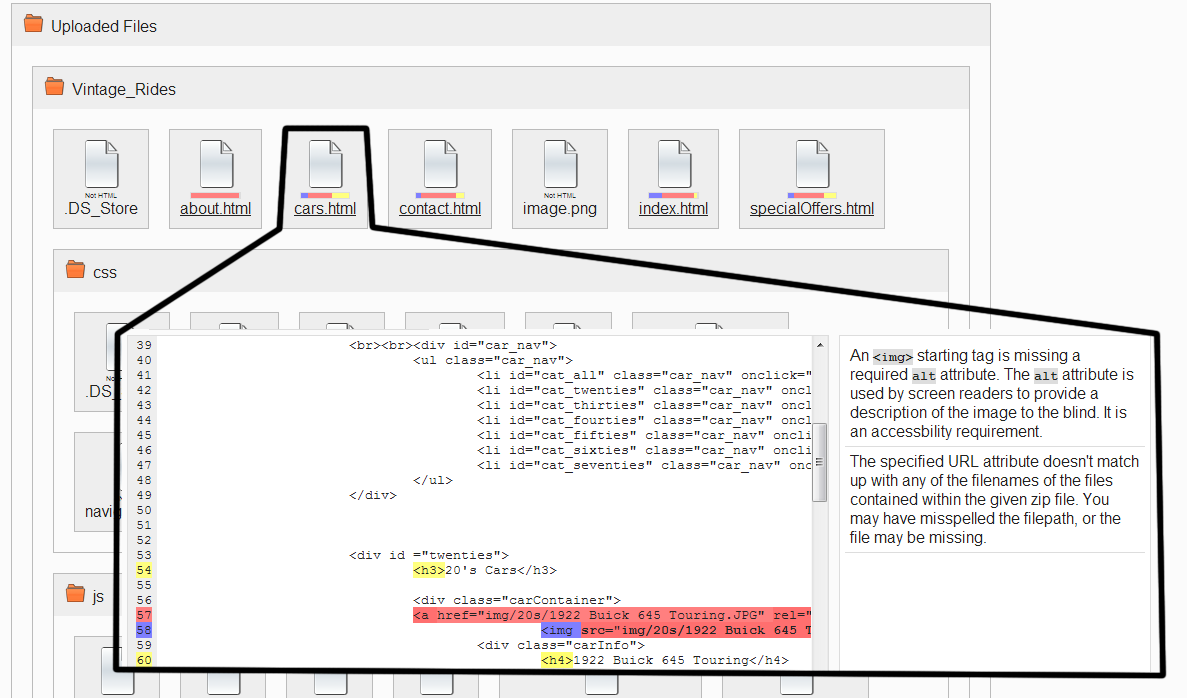
\includegraphics[scale=0.25]{file_and_broken_link.png}
\end{center}

Users can also view a file-structure view of their uploaded website zips and receive insight into any broken links their website might contain, as seen above. Any HTML files in their uploaded zip are parsed, while other non-HTML files are left unparsed.

\section*{Documentation of the Project}

The documentation provided aims to give a retrospective on the project. There are six other pieces of documentation:

\begin{enumerate}
\item User Guide - A help page presented to users to better understand how to use the website. Also available in video form.
\item Frequently Asked Questions - A list of questions that came up in development and testing that are common points of error.
\item Installation Manual - This guide aims to provide reasonable instructions as to how to install this web application on a server.
\item Updated Test Plan - A summary of all of the testing conducted, updated to include better coverage of now implemented tests.
\item Supplimentary Material - The poster used to promote this application at the demonstration.
\item Critical Evaluation and Reflection - A reflection on the project as a whole, compiled from the group's experiences and feelings on the project.
\end{enumerate}

From the \verb+README.html+ page, you can easily reach each of the files referring to these parts of documentation.

\end{document}